\documentclass[a4paper,12pt,twoside]{memoir}

% Castellano

\usepackage[spanish,es-tabla]{babel}
\selectlanguage{spanish}
\usepackage[utf8]{inputenc}
\usepackage[T1]{fontenc}
\usepackage{lmodern} % Scalable font
\usepackage{microtype}
\usepackage{placeins}

\RequirePackage{booktabs}
\RequirePackage[table]{xcolor}
\RequirePackage{xtab}
\RequirePackage{multirow}

% Links
\PassOptionsToPackage{hyphens}{url}\usepackage[colorlinks]{hyperref}
\hypersetup{
	allcolors = {red}
}

% Ecuaciones
\usepackage{amsmath}

% Rutas de fichero / paquete
\newcommand{\ruta}[1]{{\sffamily #1}}

% Párrafos
\nonzeroparskip

% Huérfanas y viudas
\widowpenalty100000
\clubpenalty100000

% Imágenes

% Comando para insertar una imagen en un lugar concreto.
% Los parámetros son:
% 1 --> Ruta absoluta/relativa de la figura
% 2 --> Texto a pie de figura
% 3 --> Tamaño en tanto por uno relativo al ancho de página
\usepackage{graphicx}
\newcommand{\imagen}[3]{
	\begin{figure}[!h]
		\centering
		\includegraphics[width=#3\textwidth]{#1}
		\caption{#2}\label{fig:#1}
	\end{figure}
	\FloatBarrier
}

% Comando para insertar una imagen sin posición.
% Los parámetros son:
% 1 --> Ruta absoluta/relativa de la figura
% 2 --> Texto a pie de figura
% 3 --> Tamaño en tanto por uno relativo al ancho de página
\newcommand{\imagenflotante}[3]{
	\begin{figure}
		\centering
		\includegraphics[width=#3\textwidth]{#1}
		\caption{#2}\label{fig:#1}
	\end{figure}
}

% El comando \figura nos permite insertar figuras comodamente, y utilizando
% siempre el mismo formato. Los parametros son:
% 1 --> Porcentaje del ancho de página que ocupará la figura (de 0 a 1)
% 2 --> Fichero de la imagen
% 3 --> Texto a pie de imagen
% 4 --> Etiqueta (label) para referencias
% 5 --> Opciones que queramos pasarle al \includegraphics
% 6 --> Opciones de posicionamiento a pasarle a \begin{figure}
\newcommand{\figuraConPosicion}[6]{%
  \setlength{\anchoFloat}{#1\textwidth}%
  \addtolength{\anchoFloat}{-4\fboxsep}%
  \setlength{\anchoFigura}{\anchoFloat}%
  \begin{figure}[#6]
    \begin{center}%
      \Ovalbox{%
        \begin{minipage}{\anchoFloat}%
          \begin{center}%
            \includegraphics[width=\anchoFigura,#5]{#2}%
            \caption{#3}%
            \label{#4}%
          \end{center}%
        \end{minipage}
      }%
    \end{center}%
  \end{figure}%
}

%
% Comando para incluir imágenes en formato apaisado (sin marco).
\newcommand{\figuraApaisadaSinMarco}[5]{%
  \begin{figure}%
    \begin{center}%
    \includegraphics[angle=90,height=#1\textheight,#5]{#2}%
    \caption{#3}%
    \label{#4}%
    \end{center}%
  \end{figure}%
}
% Para las tablas
\newcommand{\otoprule}{\midrule [\heavyrulewidth]}
%
% Nuevo comando para tablas pequeñas (menos de una página).
\newcommand{\tablaSmall}[5]{%
 \begin{table}
  \begin{center}
   \rowcolors {2}{gray!35}{}
   \begin{tabular}{#2}
    \toprule
    #4
    \otoprule
    #5
    \bottomrule
   \end{tabular}
   \caption{#1}
   \label{tabla:#3}
  \end{center}
 \end{table}
}

%
% Nuevo comando para tablas pequeñas (menos de una página).
\newcommand{\tablaSmallSinColores}[5]{%
 \begin{table}[H]
  \begin{center}
   \begin{tabular}{#2}
    \toprule
    #4
    \otoprule
    #5
    \bottomrule
   \end{tabular}
   \caption{#1}
   \label{tabla:#3}
  \end{center}
 \end{table}
}

\newcommand{\tablaApaisadaSmall}[5]{%
\begin{landscape}
  \begin{table}
   \begin{center}
    \rowcolors {2}{gray!35}{}
    \begin{tabular}{#2}
     \toprule
     #4
     \otoprule
     #5
     \bottomrule
    \end{tabular}
    \caption{#1}
    \label{tabla:#3}
   \end{center}
  \end{table}
\end{landscape}
}

%
% Nuevo comando para tablas grandes con cabecera y filas alternas coloreadas en gris.
\newcommand{\tabla}[6]{%
  \begin{center}
    \tablefirsthead{
      \toprule
      #5
      \otoprule
    }
    \tablehead{
      \multicolumn{#3}{l}{\small\sl continúa desde la página anterior}\\
      \toprule
      #5
      \otoprule
    }
    \tabletail{
      \hline
      \multicolumn{#3}{r}{\small\sl continúa en la página siguiente}\\
    }
    \tablelasttail{
      \hline
    }
    \bottomcaption{#1}
    \rowcolors {2}{gray!35}{}
    \begin{xtabular}{#2}
      #6
      \bottomrule
    \end{xtabular}
    \label{tabla:#4}
  \end{center}
}

%
% Nuevo comando para tablas grandes con cabecera.
\newcommand{\tablaSinColores}[6]{%
  \begin{center}
    \tablefirsthead{
      \toprule
      #5
      \otoprule
    }
    \tablehead{
      \multicolumn{#3}{l}{\small\sl continúa desde la página anterior}\\
      \toprule
      #5
      \otoprule
    }
    \tabletail{
      \hline
      \multicolumn{#3}{r}{\small\sl continúa en la página siguiente}\\
    }
    \tablelasttail{
      \hline
    }
    \bottomcaption{#1}
    \begin{xtabular}{#2}
      #6
      \bottomrule
    \end{xtabular}
    \label{tabla:#4}
  \end{center}
}

%
% Nuevo comando para tablas grandes sin cabecera.
\newcommand{\tablaSinCabecera}[5]{%
  \begin{center}
    \tablefirsthead{
      \toprule
    }
    \tablehead{
      \multicolumn{#3}{l}{\small\sl continúa desde la página anterior}\\
      \hline
    }
    \tabletail{
      \hline
      \multicolumn{#3}{r}{\small\sl continúa en la página siguiente}\\
    }
    \tablelasttail{
      \hline
    }
    \bottomcaption{#1}
  \begin{xtabular}{#2}
    #5
   \bottomrule
  \end{xtabular}
  \label{tabla:#4}
  \end{center}
}



\definecolor{cgoLight}{HTML}{EEEEEE}
\definecolor{cgoExtralight}{HTML}{FFFFFF}

%
% Nuevo comando para tablas grandes sin cabecera.
\newcommand{\tablaSinCabeceraConBandas}[5]{%
  \begin{center}
    \tablefirsthead{
      \toprule
    }
    \tablehead{
      \multicolumn{#3}{l}{\small\sl continúa desde la página anterior}\\
      \hline
    }
    \tabletail{
      \hline
      \multicolumn{#3}{r}{\small\sl continúa en la página siguiente}\\
    }
    \tablelasttail{
      \hline
    }
    \bottomcaption{#1}
    \rowcolors[]{1}{cgoExtralight}{cgoLight}

  \begin{xtabular}{#2}
    #5
   \bottomrule
  \end{xtabular}
  \label{tabla:#4}
  \end{center}
}



\graphicspath{ {./img/} }

% Capítulos
\chapterstyle{bianchi}
\newcommand{\capitulo}[2]{
	\setcounter{chapter}{#1}
	\setcounter{section}{0}
	\setcounter{figure}{0}
	\setcounter{table}{0}
	\chapter*{\thechapter.\enskip #2}
	\addcontentsline{toc}{chapter}{\thechapter.\enskip #2}
	\markboth{#2}{#2}
}

% Apéndices
\renewcommand{\appendixname}{Apéndice}
\renewcommand*\cftappendixname{\appendixname}

\newcommand{\apendice}[1]{
	%\renewcommand{\thechapter}{A}
	\chapter{#1}
}

\renewcommand*\cftappendixname{\appendixname\ }

% Formato de portada
\makeatletter
\usepackage{xcolor}
\newcommand{\tutor}[1]{\def\@tutor{#1}}
\newcommand{\course}[1]{\def\@course{#1}}
\definecolor{cpardoBox}{HTML}{E6E6FF}
\def\maketitle{
  \null
  \thispagestyle{empty}
  % Cabecera ----------------
\noindent
\includegraphics[width=\textwidth]{cabecera}\vspace{1cm}%
  \vfill
  % Título proyecto y escudo informática ----------------
  \colorbox{cpardoBox}{%
    \begin{minipage}{.8\textwidth}
      \vspace{.5cm}\Large
      \begin{center}
      \textbf{TFG del Grado en Ingeniería Informática}\vspace{.6cm}\\
      \textbf{\LARGE\@title{}}
      \end{center}
      \vspace{.2cm}
    \end{minipage}

  }%
  \hfill\begin{minipage}{.20\textwidth}
    
\includegraphics[width=\textwidth]{escudoInfor}
  \end{minipage}
  \vfill
  % Datos de alumno, curso y tutores ------------------
  \begin{center}%
  {%
    \noindent\LARGE
    Presentado por \@author{}\\ 
    en Universidad de Burgos --- \@date{}\\
    Tutor: \@tutor{}\\
  }%
  \end{center}%
  \null
  \cleardoublepage
  }
\makeatother

\newcommand{\nombre}{Igor Arroyo Ortega} %%% cambio de comando

% Datos de portada
\title{SugAIr: aplicación móvil proactiva para el control de niveles de insulina en diabetes}
\author{\nombre}
\tutor{Juan José Rodriguez Diez

Tutor de empresa (HP): Jose Luis Vidal de la Rosa}
\date{\today}

\begin{document}

\maketitle


\newpage\null\thispagestyle{empty}\newpage


%%%%%%%%%%%%%%%%%%%%%%%%%%%%%%%%%%%%%%%%%%%%%%%%%%%%%%%%%%%%%%%%%%%%%%%%%%%%%%%%%%%%%%%%

\thispagestyle{empty}

\noindent
\includegraphics[width=\textwidth]{cabecera}\vspace{1cm}

\noindent D. Juan José Rodríguez Diez, profesor del departamento de de Ingeniería Informática, área de Lenguajes y Sistemas Informáticos..

\noindent Expone:

\noindent Que el alumno D. \nombre, con DNI 45575268D, ha realizado el Trabajo final de Grado en Ingeniería Informática titulado SugAIr la aplicación Inteligente para dispositivos móviles que ayuda de forma proactiva a las personas con diabetes a controlar sus niveles de insulina. 

\noindent Y que dicho trabajo ha sido realizado por el alumno bajo la dirección del que suscribe, en virtud de lo cual se autoriza su presentación y defensa.

\begin{center} %\large
En Burgos, {\large \today}
\end{center}

\vfill\vfill\vfill

% Author and supervisor
\begin{minipage}{0.45\textwidth}
\begin{flushleft} %\large
Vº. Bº. del Tutor:\\[2cm]
D. Juan José Rodríguez Diez
\end{flushleft}
\end{minipage}
\hfill
\begin{minipage}{0.45\textwidth}
\begin{flushleft} %\large
\end{flushleft}
\end{minipage}
\hfill

\vfill


\newpage\null\thispagestyle{empty}\newpage




\frontmatter

% Abstract en castellano
\renewcommand*\abstractname{Resumen}
\begin{abstract}
SugAIr es una aplicación para dispositivos móviles especialmente creada y diseñada para ayudar a las personas con diabetes a centralizar y facilitar el control diario. Su objetivo principal es hacer su día a día más fácil. Busca dotar al usuario de total autonomía y conocimiento sobre su enfermedad.

El paciente cuenta con un asistente virtual con el apoyo de la Inteligencia Artificial (IA), herramientas médicas actuales y un seguimiento personalizado.
El asistente analiza rutinas y ayuda a prevenir riesgos de salud y resolve dudas respecto a la diabetes.

A nivel técnico, se apoya en una arquitectura de tres componentes: la propia app móvil, un servidor backend y modelos de lenguaje (LLM) ejecutados en local en el movil. Aunque la app está pensada para el movil tambien se puede ejecutar en el ordenador.

La tecnología empleada es React Native y el autor usó el lenguaje de programción Golong para hacer el backend
En el runtime para los modelos de IA se ha utilizado Ollama.

\end{abstract}

\renewcommand*\abstractname{Descriptores}
\begin{abstract}.
App móvil, inteligencia artificial, diabetes, React Native, API REST, Golang, asistente virtual, LLM local, educación sobre la diabetes, control glucémico, salud digital.
\end{abstract}

\clearpage

% Abstract en inglés
\renewcommand*\abstractname{Abstract}
\begin{abstract}
SugAIr is an application for mobile devices specially created and designed to help people with diabetes centralize and facilitate their daily control. Its main objective is to make their day-to-day life easier. It seeks to provide the user with total autonomy and knowledge about their disease.

The patient has a virtual assistant supported by Artificial Intelligence (AI), current medical tools, and personalized monitoring. The assistant analyzes routines and helps prevent health risks and resolve doubts regarding diabetes.

On a technical level, it relies on a three-component architecture: the mobile app itself, a backend server, and language models (LLMs) executed locally on the mobile phone. Although the app is designed for mobile, it can also be run on a computer.

The technology used is React Native and the author used the Golang programming language to build the backend. For the runtime of the AI models, Ollama has been used.
\end{abstract}

\renewcommand*\abstractname{Keywords}
\begin{abstract}
Mobile application, artificial intelligence, diabetes, React Native, REST API, Golang, virtual assistant, local LLM, diabetes education, glycemic control, digital health.
\end{abstract}

\clearpage

% Indices
\tableofcontents

\clearpage

\listoffigures

\clearpage

\listoftables
\clearpage

\mainmatter
\capitulo{1}{Introducción}
Durante las últimas décadas se ha observado un aumento considerable en el número de afectados por la diabetes. Las previsiones para 2035 coinciden en que la cifra de diabéticos se duplicará hasta alcanzar los 5,1 millones de afectados \cite{idf_atlas_diabetes}. Para los pacientes, esto supone un cambio drástico en su estilo de vida y la necesidad de un seguimiento constante. Por ello, resulta vital mantener un control exhaustivo de la enfermedad y fomentar el autoconocimiento.

Debido a las exigencias y cuidados requeridos, un control inadecuado puede derivar en la aparición de patologías asociadas. Estas complicaciones pueden afectar gravemente a órganos vitales como el corazón o los riñones, así como provocar problemas circulatorios en las extremidades o causar enfermedades oculares severas como las retinopatías.

Resulta fundamental que las personas diagnosticadas sepan gestionar su condición y dispongan de las herramientas tecnológicas adecuadas. En la actualidad existen múltiples dispositivos médicos, tales como glucómetros, sensores de medición continua de glucosa, bombas de insulina o bolígrafos inteligentes, entre otros. Sin embargo, en el panorama actual no existe un ecosistema unificado donde el usuario pueda centralizar la información y aprovechar al máximo las ventajas conjuntas que ofrecen estas herramientas. 

Adicionalmente, uno de los puntos más vulnerables en el tratamiento es la educación diabetológica. Esta responsabilidad suele estar delegada en un reducido número de especialistas dentro del entorno hospitalario. Esto provoca que el seguimiento continuado, especialmente en entornos rurales, resulte complejo y menos accesible, forzando a que el control diario y la toma de decisiones deban ser asumidos casi en su totalidad por el propio paciente.

En este contexto nace SugAIr, un proyecto cuyo objetivo es el desarrollo de un asistente conversacional inteligente diseñado para ofrecer soporte y educación diabetológica de forma accesible y privada. Mediante una aplicación web, el sistema integra Inteligencia Artificial Generativa de ejecución local. Esta decisión arquitectónica permite resolver dudas en tiempo real garantizando que la información médica sensible del usuario no abandone su propio entorno de ejecución.

Todo el código fuente del proyecto, así como el histórico de desarrollo y las versiones de los modelos empleados, están disponibles públicamente en el repositorio de GitHub del proyecto: 
\url{https://github.com/igorArroyo/TFG-de-Igor}

Del mismo modo, el seguimiento del desarrollo, la definición de iteraciones y la gestión ágil del trabajo se han administrado mediante un tablero Kanban, disponible en la plataforma GitLab:
\url{https://gitlab.com/HP-SCDS/Observatorio/2025-2026/sugair/ubu-sugair/-/boards}
(No soy el administrador de este repositorio, el que quiera acceso que me lo pida y hablo con Luis para que os de acceso)



\capitulo{2}{Objetivos del proyecto}
El objetivo principal de SugAIr es desarrollar una aplicación que sirva como núcleo central para ofrecer al paciente todo el conocimiento y las herramientas necesarias para controlar su diabetes de forma satisfactoria. A continuación, se detallan los subobjetivos que han guiado el desarrollo del proyecto, estructurados en dos niveles fundamentales:

\section{Objetivos generales}

Los propósitos principales que definen el alcance y el valor que la herramienta aportará al usuario final son los siguientes:

\begin{enumerate}
    \item \textbf{Centralizar la gestión de la enfermedad:} Aunar en una única plataforma las funciones de educación, predicción y seguimiento de la diabetes mediante el uso de Inteligencia Artificial.
    \item \textbf{Desarrollar un agente especializado:} Proveer un asistente conversacional capaz de contestar preguntas única y exclusivamente sobre diabetes, actuando como un educador diabetológico virtual.
    \item \textbf{Integrar análisis de contexto visual:} Permitir el envío y procesamiento de imágenes (por ejemplo, etiquetas de alimentos) para extraer su valor nutricional, calcular raciones de hidratos de carbono y determinar su velocidad de absorción.
    \item \textbf{Garantizar la privacidad del usuario:} Procesar las interacciones y los datos médicos de forma local, evitando la exposición de información de salud en servidores de terceros.
\end{enumerate}

\section{Objetivos técnicos}

Para alcanzar las metas funcionales establecidas, se han definido los siguientes objetivos a nivel de arquitectura e implementación tecnológica:

\begin{enumerate}
    \item \textbf{Implementar una arquitectura cliente-servidor desacoplada:} Desarrollar un frontend dinámico mediante React (utilizando el entorno Expo) que consuma una API REST construida con el lenguaje Go.
    \item \textbf{Integrar un motor de Inteligencia Artificial local:} Emplear Ollama como entorno de ejecución para desplegar Modelos de Lenguaje Grande (LLM) con capacidades multimodales (procesamiento de texto e imagen) en el propio hardware del servidor.
    \item \textbf{Construir una interfaz de usuario reactiva:} Diseñar una aplicación web inspirada en plataformas de mensajería (chat), priorizando la fluidez y la experiencia de uso en la interacción en tiempo real.
    \item \textbf{Aplicar metodologías ágiles:} Gestionar el ciclo de vida del desarrollo mediante sprints de tres semanas apoyadas en un tablero Kanban.
\end{enumerate}
\capitulo{3}{Conceptos teóricos}

En este capítulo se exponen los fundamentos médicos y biológicos necesarios para comprender la naturaleza de la diabetes mellitus y su tratamiento diario. El conocimiento riguroso de la fisiología celular, los tipos de diabetes, los riesgos asociados a las alteraciones glucémicas y las pautas de insulinización resulta imprescindible para justificar las funcionalidades predictivas y educativas implementadas en el asistente conversacional SugAIr.

\section{Fisiología celular básica: la glucosa y la energía}
El cuerpo humano está compuesto por billones de células, que son las unidades anatómicas y funcionales fundamentales de los seres vivos. Para que una célula pueda realizar sus funciones (como la contracción muscular o la transmisión de impulsos nerviosos), necesita energía. Esta energía se obtiene principalmente a través de un proceso químico que transforma los alimentos en una molécula llamada ATP (Trifosfato de Adenosina), que actúa como la moneda energética del organismo \cite{medline_celula}.

El principal combustible que utilizan las células para fabricar este ATP es la glucosa. La glucosa es un monosacárido, es decir, la forma más simple de los hidratos de carbono (azúcares y almidones presentes en los alimentos). Tras la digestión, estos hidratos de carbono se descomponen y la glucosa pasa al torrente sanguíneo. El índice de glucosa en sangre representa, por tanto, el nivel de azúcar circulante. Este combustible es especialmente crítico para el cerebro, el cual necesita azúcar de forma constante para funcionar adecuadamente \cite{guyton2021}.

\section{¿Qué es la diabetes?}
La diabetes mellitus (DM) comprende un grupo de trastornos metabólicos crónicos cuya característica fisiopatológica principal común es la hiperglucemia (niveles crónicamente elevados de glucosa en el plasma sanguíneo). Esta condición patológica se deriva de alteraciones en la secreción de insulina, en la acción biológica de dicha hormona a nivel tisular, o en una combinación de ambas.

La insulina es una hormona anabólica secretada por las células beta pancreáticas (ubicadas en los islotes de Langerhans), cuya función primordial es facilitar la captación celular de la glucosa circulante para su metabolismo o almacenamiento. La desregulación de este mecanismo provoca que la glucosa no pueda penetrar eficazmente en las células, acumulándose en el torrente sanguíneo. A largo plazo, esta hiperglucemia sostenida genera disfunción y daño orgánico, afectando especialmente al sistema vascular, los riñones, la retina y el sistema nervioso periférico \cite{revespcardiol_diabetes}.

\section{Síntomas de la diabetes}
La sintomatología clínica clásica de la diabetes mellitus está directamente fundamentada en las alteraciones producidas por la hiperglucemia severa. Los síntomas cardinales, frecuentemente denominados en la literatura clínica como la ``regla de las 4 P'', incluyen los siguientes \cite{who_diabetes, nutriwhite_4p}:

\begin{itemize}
    \item \textbf{Poliuria}: Excreción excesiva de orina. Ocurre cuando la concentración de glucosa sérica supera el umbral renal de reabsorción. El exceso de glucosa se excreta en la orina, arrastrando consigo agua por ósmosis, lo que provoca una diuresis osmótica.
    \item \textbf{Polidipsia}: Sed excesiva. Consiste en un mecanismo fisiológico compensatorio; la pérdida masiva de líquidos a través de la poliuria genera una deshidratación que activa los osmorreceptores hipotalámicos, induciendo la sensación de sed.
    \item \textbf{Polifagia}: Aumento desmesurado del apetito. A pesar de la abundancia de glucosa en sangre, el déficit de insulina impide que esta penetre en las células, generando un estado de inanición celular que el cerebro interpreta como falta de alimento.
    \item \textbf{Pérdida de peso inexplicable}: Debido a la incapacidad de utilizar la glucosa como sustrato energético principal, el organismo recurre a vías metabólicas alternativas, desencadenando el catabolismo de triglicéridos en el tejido adiposo y de proteínas en el músculo esquelético.
\end{itemize}

\section{Tipos de diabetes}
La etiología de la diabetes mellitus es heterogénea. La clasificación contemporánea se basa fundamentalmente en la patogenia y el origen del trastorno, categorizándose en cuatro grandes grupos principales \cite{who_diabetes}:

\begin{enumerate}
    \item \textbf{Diabetes Tipo 1}: Mediada por la destrucción de las células beta.
    \item \textbf{Diabetes Tipo 2}: Caracterizada por la resistencia a la insulina y el déficit progresivo de su secreción.
    \item \textbf{Diabetes Mellitus Gestacional (DMG)}: Hiperglucemia diagnosticada por primera vez durante el embarazo.
    \item \textbf{Tipos específicos por otras causas}: Síndromes genéticos, patologías del páncreas exocrino o diabetes inducida por fármacos.
\end{enumerate}

\subsection{Diabetes Tipo 1}
La diabetes mellitus tipo 1 representa una minoría de los casos globales. Su rasgo patogénico definitorio es la destrucción progresiva e irreversible de las células beta del páncreas, lo que conduce a un déficit absoluto en la secreción de insulina \cite{revespcardiol_diabetes}. 

Los pacientes con este diagnóstico son insulinodependientes de forma absoluta a lo largo del día \cite{ada_standards}. En las primeras fases de la enfermedad, es necesario tener en cuenta las denominadas fases de luna de miel, en las que el páncreas conserva capacidad residual para generar insulina de forma natural, lo que puede provocar episodios de hipoglucemia a consecuencia de la inyección superpuesta de insulina artificial \cite{cinfasalud_diabetes}.

\subsection{Diabetes Tipo 2}
La diabetes mellitus tipo 2 es la variante clínica más prevalente. Su patogenia es compleja y de naturaleza bifásica, caracterizándose por la coexistencia de resistencia a la insulina y una disfunción progresiva de las células beta pancreáticas. 

La resistencia a la insulina implica una respuesta biológica subóptima a esta hormona. En las etapas precoces, el páncreas logra compensar esta resistencia secretando cantidades supranormales de insulina. Sin embargo, con el transcurso del tiempo, las células beta sufren estrés oxidativo, claudican y se vuelven incapaces de mantener esta hipersecreción, instaurándose un déficit relativo de insulina. A lo largo del día, una misma persona puede ofrecer diferentes niveles de resistencia a la insulina, lo que significa que la cantidad de unidades necesarias para metabolizar una misma ingesta de hidratos de carbono puede variar en función de la hora, siendo un patrón que suele mantenerse constante en el propio paciente \cite{doctorsolano_hiperinsulinemia}.

\section{Control glucémico y complicaciones agudas}
En el control diario de la enfermedad, se establece que un nivel aceptable de azúcar en sangre se encuentra dentro del rango de 70 a 120 mg/dl \cite{ada_standards, idf_atlas_diabetes}. Las desviaciones fuera de estos parámetros conllevan riesgos graves para la salud:

\begin{itemize}
    \item \textbf{Hipoglucemia}: Se produce cuando los niveles descienden por debajo de 70 mg/dl \cite{idf_atlas_diabetes}. Ante la falta de azúcar, indispensable para el funcionamiento cerebral, se puede producir una pérdida de conocimiento que impide la ingesta de azúcares de absorción rápida, pudiendo derivar en un coma diabético \cite{ada_standards}.
    \item \textbf{Hiperglucemia}: Ocurre cuando los niveles superan los 120 mg/dl \cite{idf_atlas_diabetes}. Sin el tratamiento insulínico correcto, el cuerpo recurre a la obtención de energía a partir de la grasa corporal, un proceso que genera cuerpos cetónicos \cite{ada_standards}. Estos compuestos orgánicos son tóxicos en altas cantidades y pueden provocar cetoacidosis, una complicación severa que, ante la carencia de insulina, requiere el ingreso inmediato en la UCI por complicaciones cardíacas o cerebrales \cite{revespcardiol_diabetes}.
\end{itemize}

\section{Nutrición y pautas de insulinización}
La variación del azúcar en sangre depende directamente de la actividad física y de la alimentación \cite{who_diabetes}. La ingesta de hidratos de carbono se clasifica en tres tipos según su índice de absorción:

\begin{itemize}
    \item \textbf{De absorción lenta}: Cereales, harinas, pastas, legumbres y arroces \cite{cinfasalud_diabetes}.
    \item \textbf{De absorción rápida}: Azúcar refinado, zumos y miel \cite{cinfasalud_diabetes}.
    \item \textbf{De absorción semirrápida}: Frutas \cite{cinfasalud_diabetes}.
\end{itemize}

Para metabolizar estas ingestas y mantener un índice glucémico estable, el paciente insulinodependiente recurre a distintos tipos de insulina artificial \cite{ada_standards}. Las terapias actuales utilizan principalmente tres variantes:

\begin{enumerate}
    \item \textbf{Insulina lenta o basal}: Tiene una duración aproximada de 24 horas y se aplica, por norma general, una vez al día para controlar el azúcar en sangre durante el sueño, en ayunas y entre comidas \cite{ada_standards}.
    \item \textbf{Insulina rápida}: Comienza a hacer efecto entre los 5 y 15 minutos de su aplicación, alcanzando su pico máximo entre 1 y 2 horas \cite{ada_standards}. Se administra al menos tres veces al día, justo antes de las comidas principales o para corregir picos de azúcar descontrolados \cite{ada_standards}.
    \item \textbf{Insulina de acción intermedia}: Comienza a hacer efecto entre 1 y 2 horas tras su inyección, con un pico máximo a partir de la cuarta a sexta hora, requiriendo un mayor número de aplicaciones diarias que la insulina basal \cite{ada_standards}.
\end{enumerate}
\capitulo{4}{Técnicas y herramientas}

Este capítulo presenta las técnicas metodológicas y las herramientas de desarrollo empleadas para la implementación de SugAIr. Siguiendo las directrices del proyecto, se enumeran las tecnologías de uso común empleadas en la arquitectura base y se detallan con mayor profundidad aquellas soluciones novedosas, como la ejecución local de modelos de Inteligencia Artificial, justificando en cada caso la elección realizada frente a otras alternativas.

\section{Desarrollo del frontend: React Native}
React Native es un framework de código abierto publicado por Meta que permite el desarrollo de aplicaciones móviles utilizando la biblioteca React y el lenguaje JavaScript, compartiendo una única base de código \cite{react_native_dev}. A diferencia de otras soluciones híbridas que emplean vistas web (WebViews), esta tecnología renderiza componentes nativos, ofreciendo un rendimiento superior a nivel de interfaz.

Su arquitectura interna se basa en los siguientes componentes principales \cite{react_native_dev}:
\begin{itemize}
    \item \textbf{Código nativo y JavaScriptCore VM}: Combina módulos nativos de la plataforma con una máquina virtual subyacente que interpreta el código JavaScript en tiempo real.
    \item \textbf{React Native Bridge}: Actúa como puente de comunicación asíncrona entre el hilo de JavaScript y las APIs nativas del dispositivo.
    \item \textbf{Virtual DOM}: Consiste en una representación abstracta de la interfaz de usuario. El sistema calcula las diferencias tras cada cambio de estado y actualiza únicamente los elementos necesarios, optimizando los recursos del sistema.
\end{itemize}

\section{Desarrollo del backend: Go (Golang)}
Para la construcción del servidor y la lógica de negocio se ha optado por Go (Golang), un lenguaje de programación compilado, concurrente y de código abierto desarrollado originalmente por Google \cite{donovan_go}. Su elección frente a otros lenguajes se justifica por su alta velocidad de ejecución y su excepcional manejo de la concurrencia a través de \textit{goroutines}.

Las principales ventajas que justifican la adopción de Go en este proyecto incluyen las siguientes \cite{donovan_go}:
\begin{itemize}
    \item \textbf{Concurrencia nativa}: Facilita el desarrollo de servicios web altamente escalables permitiendo la ejecución de múltiples tareas en paralelo con un bajo consumo de memoria.
    \item \textbf{Eficiencia y rendimiento}: Al ser un lenguaje compilado directamente a código máquina, optimiza la velocidad de respuesta, característica crítica para intermediar entre el cliente y el motor de inteligencia artificial.
    \item \textbf{Sintaxis limpia y mantenibilidad}: Su diseño coherente y estricto reduce los riesgos de errores y facilita el mantenimiento a largo plazo.
    \item \textbf{Gestión de memoria}: Incorpora un recolector de basura (\textit{garbage collector}) altamente optimizado que previene fugas de memoria durante ejecuciones continuadas.
\end{itemize}

\section{Inteligencia Artificial y Modelos de Lenguaje (LLM)}
La Inteligencia Artificial (IA) generativa constituye el núcleo funcional de SugAIr, superando el enfoque de los sistemas de software tradicionales para ofrecer capacidades de razonamiento y procesamiento de lenguaje natural \cite{iso_ia}. Dada la naturaleza del proyecto, se requiere la combinación de Reconocimiento Óptico de Caracteres (OCR) con IA multimodal para extraer y estructurar datos provenientes de imágenes de manera automatizada.

Para garantizar la privacidad absoluta de los datos médicos del usuario, se ha descartado el uso de APIs de terceros en la nube, optando por la ejecución local de Modelos de Lenguaje Grande (LLM). Para este fin se emplea la herramienta Ollama \cite{ollama_official}.

Ollama es un entorno de ejecución de código abierto que presenta características fundamentales para el proyecto \cite{ollama_official, osl_ollama}:
\begin{itemize}
    \item \textbf{Privacidad y seguridad}: Permite descargar y ejecutar modelos directamente en el hardware local, garantizando que ninguna información sensible del paciente abandone su equipo.
    \item \textbf{Accesibilidad}: Simplifica el complejo proceso de configuración y despliegue de modelos de IA, encapsulando las dependencias técnicas.
    \item \textbf{Flexibilidad multimodal}: Permite la integración fluida de modelos capaces de procesar tanto texto como imágenes, cubriendo los requerimientos específicos de la aplicación.
\end{itemize}

\section{Arquitectura API REST}
La comunicación entre la aplicación cliente y el servidor se realiza mediante una arquitectura basada en el estilo arquitectónico API REST, introducido formalmente por Roy Fielding \cite{fielding_rest}. Este estándar de desarrollo garantiza la interoperabilidad, la escalabilidad y la separación de responsabilidades.

La implementación de esta arquitectura en el proyecto se fundamenta en los siguientes principios:
\begin{itemize}
    \item \textbf{Independencia Cliente-Servidor}: El frontend y el backend pueden evolucionar y escalar de forma totalmente independiente.
    \item \textbf{Sistema por capas y modularidad}: Permite que las peticiones fluyan a través de diferentes intermediarios (como el servidor en Go y el motor de inferencia Ollama) de forma transparente para el usuario final.
    \item \textbf{Endpoints y métodos HTTP}: Se definen rutas específicas gobernadas por verbos estándar (GET, POST, PUT, DELETE) para el intercambio de información.
\end{itemize}

\section{Gestión del proyecto: GitLab y Control de Versiones}
Para la administración del ciclo de vida del desarrollo se ha utilizado la plataforma GitLab, unificando la planificación de tareas y la custodia del código fuente bajo el paradigma de entrega ágil \cite{gitlab_agile}.

La metodología de trabajo se apoya en las siguientes herramientas integradas:
\begin{itemize}
    \item \textbf{Tableros Kanban}: Proporcionan una visualización clara del flujo de trabajo, dividiendo las iteraciones en tareas (\textit{issues}) que transitan por distintos estados (pendientes, en proceso, finalizadas), facilitando el control continuo y limitando el trabajo en curso \cite{anderson_kanban, gitlab_kanban}.
    \item \textbf{Control de versiones (Git)}: Garantiza la trazabilidad absoluta del código. Cada modificación queda registrada con su autor y fecha, permitiendo la creación de ramas aisladas para nuevas funciones y posibilitando la reversión a versiones estables en caso de fallo crítico \cite{gitlab_version_control}.
\end{itemize}
\capitulo{5}{Aspectos relevantes del desarrollo del proyecto}

Este capítulo pretende recoger los aspectos más destacados y las decisiones de diseño adoptadas durante el ciclo de vida de SugAIr. En lugar de realizar una descripción exhaustiva del código fuente, se documentan los caminos de solución elegidos ante los retos técnicos planteados, con especial énfasis en la arquitectura del sistema, el ciclo de trabajo ágil y la integración del modelo de Inteligencia Artificial local.



\section{Inicio del proyecto y metodología de trabajo}
El origen del proyecto surge de la colaboración entre la Universidad de Burgos y el Programa Observatorio Tecnológico HP SCDS. A partir de los requisitos iniciales, se estableció un flujo de trabajo ágil apoyado en la plataforma GitLab, lo que permitió abandonar el desarrollo no estructurado en favor de un control iterativo basado en entregas de valor.

El progreso se dividió en ciclos de trabajo (sprints) gestionados mediante un tablero Kanban, garantizando la trazabilidad de cada tarea (\textit{issue}). A nivel organizativo, las primeras fases del desarrollo se estructuraron de la siguiente manera:

\begin{itemize}
    \item \textbf{Sprint 1: Preparación del entorno.} Dedicado a la instalación y configuración de las herramientas base del ecosistema, incluyendo VSCode, el entorno de React Native y el compilador de Go.
    \item \textbf{Sprint 2: Pruebas de concepto y esqueleto.} Generación de los primeros \textit{endpoints} de validación (healthcheck) en el servidor y creación del proyecto base en el frontend para establecer la comunicación inicial.
    \item \textbf{Sprint 3: Despliegue de IA local.} Fase de investigación orientada a la descarga de Ollama y la búsqueda de modelos de lenguaje compatibles con las especificaciones de hardware del equipo de desarrollo.
    \item \textbf{Sprint 4: Integración y control de la IA.} Establecimiento de las peticiones HTTP desde el servidor Go hacia Ollama, creación de la interfaz de chat en React y aplicación de ingeniería de \textit{prompts} para restringir las respuestas del modelo.
    \item \textbf{Sprint 5: Modelo multimodal, documentación y cierre.} Investigaición e implementación de un modelo multimodal y adaptación de la UI para adjuntar imágenes.
    Tambien acabar la documentación.
\end{itemize}
\clearpage
\begin{figure}
    \centering
    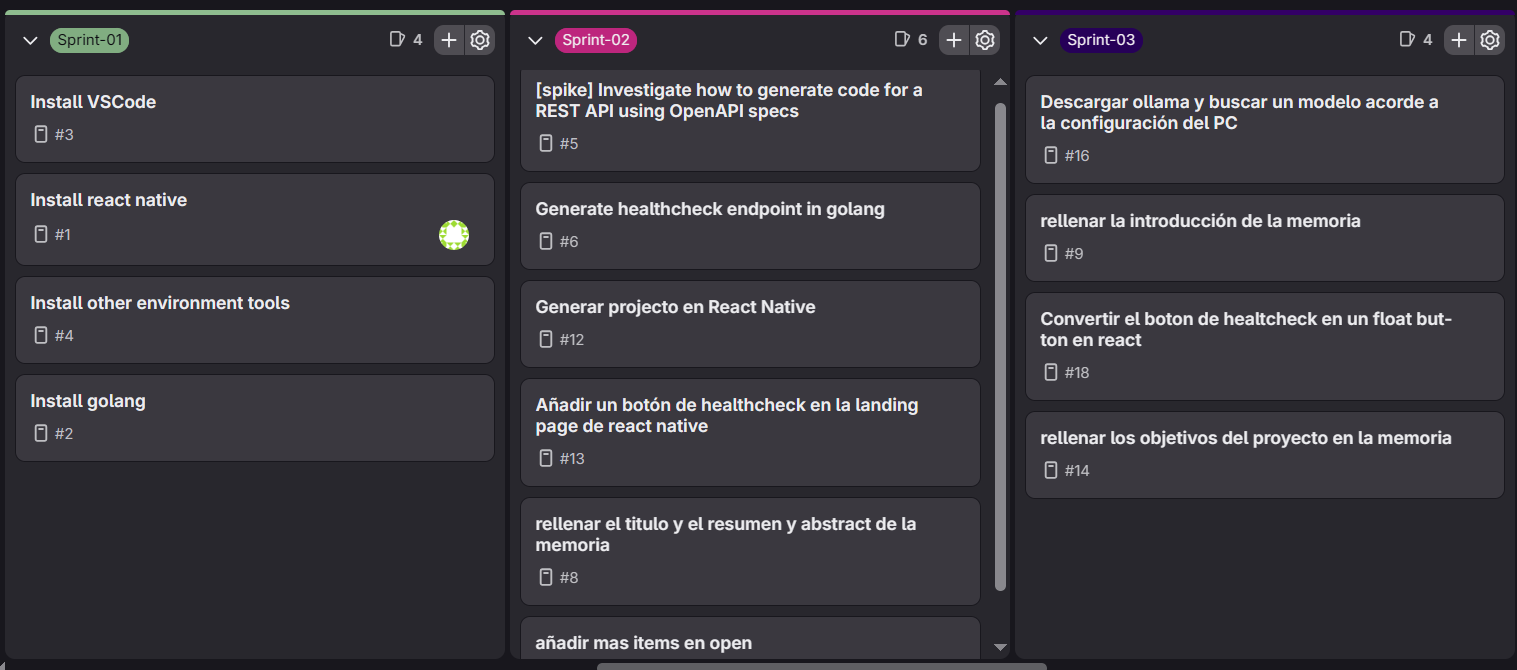
\includegraphics[width=0.75\linewidth]{tablero1.png}
    \caption{Sprints 1-3 en el tablero kanban}
    \label{fig:tablero1}
\end{figure}

\begin{figure}
    \centering
    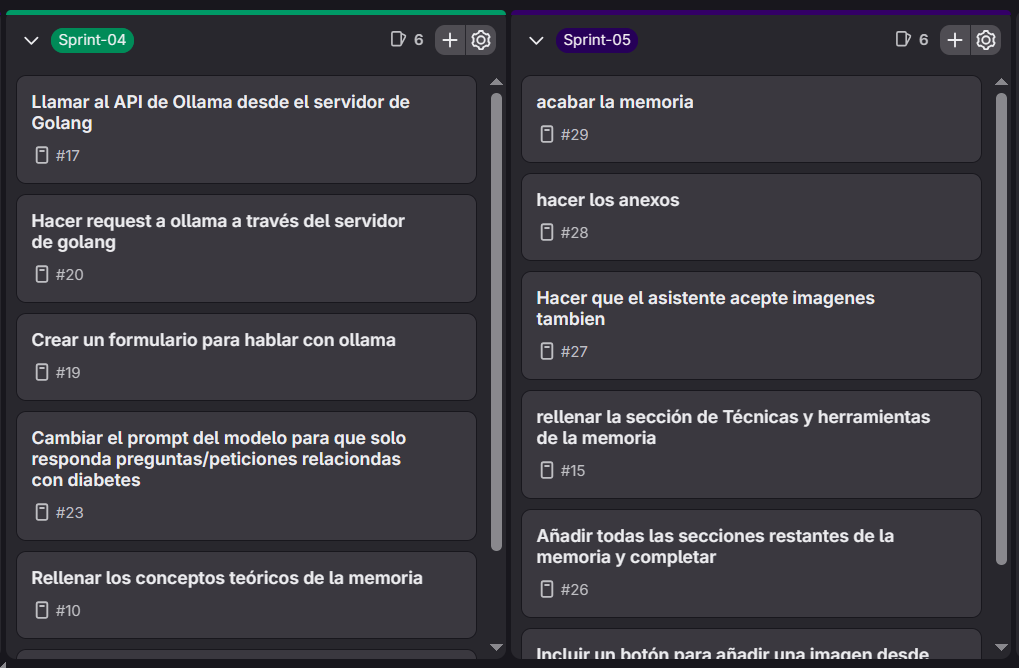
\includegraphics[width=0.75\linewidth]{tablero2.png}
    \caption{sprints 4-5}
    \label{fig:tablero2}
\end{figure}
\clearpage

\section{Desarrollo y arquitectura del backend}
El núcleo de la lógica de negocio y la gestión de peticiones reside en un servidor backend desarrollado en Go. Su función principal es actuar como una capa de seguridad y orquestación.

Para la comunicación con el motor de Inteligencia Artificial, se descartó la implementación de integraciones complejas basadas en librerías de terceros, optando por una solución más limpia y mantenible: el uso de peticiones HTTP directas contra la API REST que expone Ollama en el entorno local (localhost). Este diseño convierte al servidor en Go en un intermediario (proxy) que recibe los datos del frontend, lo formatea adecuadamente inyectando las directrices del sistema, y lo envía al modelo. 

Esta arquitectura presenta una ventaja crítica: si en el futuro se decide migrar de Ollama a otro entorno de ejecución local (como vLLM o llama.cpp), la aplicación cliente no sufrirá ningún impacto, ya que la adaptación se realizará de forma transparente y centralizada en el servidor Go.

\section{El problema de la ejecución local y las restricciones de hardware}
La integración de Modelos de Lenguaje Grande (LLM) supuso el mayor desafío técnico del proyecto. El objetivo inicial contemplaba el uso del modelo Llama 3.2 en su variante multimodal, con el fin de procesar tanto las consultas textuales del usuario como imágenes adjuntas (por ejemplo, gráficas de glucosa o etiquetas de alimentos).


Sin embargo, durante la fase de análisis (\textit{Sprint} 3), se evidenció un cuello de botella crítico: los requerimientos para la carga de un modelo base con capacidades de visión artificial excedían la memoria RAM disponible en el entorno de ejecución inicial. 

Para solventar esta limitación técnica sin comprometer el requisito fundamental de privacidad y ejecución local, se analizó el ecosistema de modelos optimizados, optando finalmente por la implementación de \textbf{Llava} (\textit{Large Language and Vision Assistant}) gestionado a través del motor Ollama. La viabilidad de esta integración radica en las técnicas de cuantización de pesos neuronales que emplea dicha plataforma, las cuales reducen drásticamente la huella en memoria del modelo permitiendo su despliegue en \textit{hardware} de consumo estándar sin una pérdida significativa de capacidad deductiva.

La elección de Llava se fundamenta en su arquitectura de vanguardia, la cual integra un codificador visual basado en la tecnología CLIP con el potente modelo de lenguaje LLaMA. Esta fusión permite al sistema interpretar de manera conjunta instrucciones semánticas y matrices de píxeles, resultando idóneo para la lectura y compresión de etiquetas nutricionales complejas.

Para adaptar esta herramienta al contexto médico del proyecto, se desarrolló una variante específica denominada \texttt{llava-diabetes}. A través de la configuración de un archivo nativo (\textit{Modelfile}), se empaquetó el modelo base cuantizado junto con un mapa de directrices (\textit{system prompt}). Este contexto preinyectado restringe el ámbito de actuación del asistente, asegura un tono profesional e impersonal, y estandariza la extracción de macronutrientes, superando así las restricciones de \textit{hardware} iniciales y consolidando un flujo multimodal robusto.

Adicionalmente, para dotar al modelo de utilidad clínica real, se aplicaron técnicas de ingeniería de contexto (\textit{prompt engineering}). Se configuró el comportamiento base del modelo para que actúe estrictamente como un educador diabetológico, programándolo para rechazar de forma controlada y segura cualquier consulta o interacción que no esté directamente relacionada con la diabetes.

\section{Desarrollo del frontend}
La capa de presentación se implementó mediante React, configurado para ejecutarse en un entorno web simulando una disposición móvil.

La interfaz principal consta de una aplicación de página única (\textit{Single Page Application}) que emula el comportamiento de plataformas de mensajería instantánea. Se han utilizado componentes dinámicos para el renderizado de chat, la entrada de texto y el manejo de los estados de carga (\textit{loading states}) mientras el servidor aguarda la inferencia generada por la Inteligencia Artificial.

\begin{figure}
    \centering
    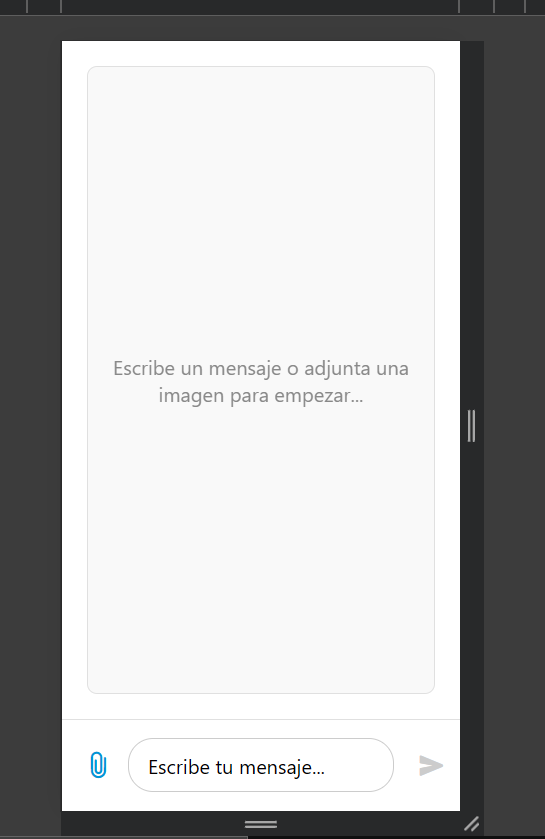
\includegraphics[width=0.75\linewidth]{frontend.png}
    \caption{pantalla inicial de la interfaz gráfica}
    \label{fig:placeholder}
\end{figure}
\capitulo{6}{Trabajos relacionados}

En el ecosistema del software orientado a la salud digital y, más específicamente, al manejo de la diabetes, se observan dos líneas de desarrollo predominantes: por un lado, las aplicaciones móviles de registro y seguimiento de datos médicos; y por otro, los asistentes virtuales de salud basados en Inteligencia Artificial. Con el objetivo de situar este proyecto en el panorama tecnológico actual, a continuación se describen tres plataformas representativas del sector y se analizan sus características frente a SugAIr.

\section{mySugr}
La plataforma mySugr \cite{mysugr} es una de las aplicaciones de gestión de la diabetes más populares a nivel global. Su funcionalidad principal reside en actuar como un cuaderno de bitácora digital (\textit{logbook}) donde los usuarios pueden registrar sus niveles de glucosa, ingesta de carbohidratos y dosis de insulina. Destaca por su enfoque en la gamificación para motivar al paciente y por su capacidad para integrarse por Bluetooth con diversos glucómetros del mercado.

Si bien mySugr es una herramienta robusta para el seguimiento de métricas y la estimación de la hemoglobina glicosilada (HbA1c), carece de un motor de Inteligencia Artificial generativa que permita al usuario interactuar mediante lenguaje natural para resolver dudas complejas de educación diabetológica en tiempo real.

\section{S.A.R.A.H. (Organización Mundial de la Salud)}
S.A.R.A.H. (Smart AI Resource Assistant for Health) \cite{sarah_who} es un promotor de salud digital impulsado por Inteligencia Artificial generativa y desarrollado por la Organización Mundial de la Salud (OMS). Este agente conversacional está diseñado para interactuar con los usuarios y proporcionar información sobre diversos temas de salud, incluyendo hábitos de vida saludables y prevención de enfermedades crónicas.

Aunque comparte con SugAIr el concepto de asistente conversacional para la educación en salud, S.A.R.A.H. es un sistema de propósito general alojado en servidores externos (en la nube). Esto implica que las interacciones de voz y texto se procesan fuera del entorno del usuario, un enfoque que difiere de la arquitectura de privacidad estricta y ejecución local planteada en este proyecto.

\section{SocialDiabetes}
SocialDiabetes \cite{socialdiabetes} es una plataforma integral de origen español, certificada como producto sanitario (\textit{Medical Device}), orientada al control de la diabetes tipo 1 y tipo 2. Permite el cálculo de dosis de insulina, la monitorización de pautas alimentarias y la conexión remota entre el paciente y el profesional sanitario a través de un panel de control en la nube.

A diferencia de SugAIr, el enfoque de SocialDiabetes es puramente clínico y de monitorización algorítmica. No integra modelos de lenguaje grande (LLM) que permitan mantener una conversación abierta y dinámica con el paciente para ofrecer consejos proactivos o explicar conceptos teóricos de forma personalizada.

\section{Comparativa sobre las funcionalidades cubiertas}

Para clarificar el valor añadido de SugAIr frente a las soluciones existentes, se presenta una tabla comparativa que evalúa las funcionalidades clave de cada sistema. El objetivo de SugAIr no es sustituir a los dispositivos médicos certificados, sino complementar el ecosistema ofreciendo un entorno privado de consulta interactiva.

\begin{table}[htbp]
\centering
\caption{Comparativa de características entre aplicaciones orientadas a la salud}
\vspace{0.2cm}
\begin{tabular}{|l|c|c|c|c|}
\hline
\textbf{Funcionalidad} & \textbf{mySugr} & \textbf{S.A.R.A.H.} & \textbf{SocialDiabetes} & \textbf{SugAIr} \\ \hline
Registro de glucosa y datos & Sí & No & Sí & No \\ \hline
IA Conversacional generativa & No & Sí & No & Sí \\ \hline
Educación diabetológica & Parcial & Sí & Parcial & Sí \\ \hline
Ejecución local (Privacidad) & No & No & No & Sí \\ \hline
Cálculo de insulina algorítmico& Sí & No & Sí & No \\ \hline
\end{tabular}
\label{tab:comparativa_apps}
\end{table}

Como se puede observar en la Tabla \ref{tab:comparativa_apps}, el valor diferencial de SugAIr radica en la combinación de un agente conversacional especializado exclusivamente en diabetes con una arquitectura de ejecución local. Mientras que las aplicaciones tradicionales se centran en el registro de datos, y los asistentes globales operan en la nube, SugAIr se posiciona como una herramienta educativa privada, sentando las bases para futuras integraciones multimodales sin comprometer los datos médicos del paciente.

%Este apartado sería parecido a un estado del arte de una tesis o tesina. En un trabajo final grado no parece obligada su presencia, aunque se puede dejar a juicio del tutor el incluir un pequeño resumen comentado de los trabajos y proyectos ya realizados en el campo del proyecto en curso. 

\capitulo{7}{Conclusiones y Líneas de trabajo futuras}

El desarrollo de este Trabajo Fin de Grado ha permitido abarcar el ciclo de vida completo de una solución de \textit{software}, desde su concepción inicial hasta su implementación final. A continuación, se detallan las conclusiones extraídas, categorizadas según los resultados obtenidos y los aspectos técnicos del desarrollo, finalizando con un análisis crítico que fundamenta las vías de continuidad del proyecto.

\section{Conclusiones del proyecto}

\subsection{Conclusiones relacionadas con los resultados}
\begin{itemize}
    \item \textbf{Viabilidad y pertinencia clínica:} Se ha logrado desarrollar una aplicación móvil completamente funcional que responde a una necesidad latente en el ámbito de la salud: dotar a los pacientes diabéticos de una herramienta privada capaz de analizar información nutricional y ofrecer soporte educativo continuo.
    \item \textbf{Cumplimiento de objetivos:} La aplicación desarrollada satisface las premisas iniciales del proyecto. Destaca especialmente la capacidad del sistema para interpretar, procesar y desglosar el impacto glucémico a partir de fotografías de etiquetas alimentarias, validando el concepto inicial de asistencia automatizada.
    \item \textbf{Privacidad por diseño (\textit{Privacy by Design}):} Al delegar el procesamiento de la Inteligencia Artificial a un entorno de ejecución local en lugar de depender de servicios en la nube (\textit{Cloud computing}), se ha garantizado la total confidencialidad de los datos médicos del usuario, cumpliendo con los estándares éticos exigibles en aplicaciones de \textit{eHealth}.
\end{itemize}

\subsection{Conclusiones técnicas}
\begin{itemize}
    \item \textbf{Arquitectura de alto rendimiento:} La integración de React Native (vía Expo) para la interfaz móvil y de Go (mediante el \textit{framework} Echo) para el servidor ha demostrado constituir una pila tecnológica altamente eficiente, garantizando un flujo de comunicación rápido, asíncrono y desacoplado.
    \item \textbf{Inteligencia Artificial Multimodal Local:} Se ha validado empíricamente la viabilidad de ejecutar Modelos de Lenguaje Grande con capacidades de visión computacional en entornos locales. Mediante la personalización del modelo base Llava (creando la variante \texttt{llava-diabetes}), se ha comprobado que la aplicación de técnicas de ingeniería de contexto (\textit{prompt engineering}) es altamente efectiva para mitigar alucinaciones algorítmicas y acotar las respuestas al marco clínico de la diabetes.
    \item \textbf{Adopción de metodologías ágiles:} El empleo de metodologías de desarrollo ágil, materializado en el uso de tableros Kanban (GitLab) y ciclos iterativos (\textit{sprints}), ha resultado decisivo para sortear bloqueos técnicos, priorizar requerimientos funcionales y asegurar una entrega de valor constante a pesar de las limitaciones temporales.
\end{itemize}

\section{Líneas de trabajo futuras}

Actualmente, la inferencia de Inteligencia Artificial en local exige un consumo intensivo de recursos de \textit{hardware}, lo que podría restringir su viabilidad en dispositivos móviles de especificaciones limitadas.

Para solventar estas carencias y potenciar el alcance de la herramienta, se proponen las siguientes líneas de trabajo futuras:

\begin{itemize}
    %\item \textbf{Sistema de persistencia y perfiles clínicos:} Acoplamiento de un motor de base de datos relacional para dotar al sistema de memoria histórica. Esto posibilitaría la creación de perfiles de usuario (almacenando el tipo de diabetes, pautas de insulina y nivel de actividad física) para generar respuestas deterministas y altamente personalizadas.
    \item \textbf{Interacción conversacional por voz (STT/TTS):} Integración de motores de conversión de voz a texto (\textit{Speech-to-Text}) y de texto a voz (\textit{Text-to-Speech}). Considerando que las consultas nutricionales suelen realizarse durante la manipulación de alimentos, la interacción mediante comandos de voz mejoraría drásticamente la ergonomía y accesibilidad de la plataforma.
    \item \textbf{Predicción algorítmica de curvas de glucosa:} Desarrollo de modelos de \textit{machine learning} clásicos (basados en análisis de series temporales) que complementen a la IA generativa. Esto permitiría correlacionar el análisis nutricional actual con predicciones glucémicas a dos horas vista, facilitando la prevención de episodios de hiperglucemia o hipoglucemia.
    \item \textbf{Integración de datos heterogéneos y sensorización:} Establecimiento de flujos de conexión con APIs externas (meteorología, bases de datos nutricionales globales) y posible lectura de datos provenientes de dispositivos de Monitorización Continua de Glucosa (MCG) y \textit{wearables} de actividad física, lo que dotaría al modelo \texttt{llava-diabetes} de un contexto clínico holístico en tiempo real.
\end{itemize}

%Todo proyecto debe incluir las conclusiones que se derivan de su desarrollo. Éstas pueden ser de diferente índole, dependiendo de la tipología del proyecto, pero normalmente van a estar presentes un conjunto de conclusiones relacionadas con los resultados del proyecto y un conjunto de conclusiones técnicas. Además, resulta muy útil realizar un informe crítico indicando cómo se puede mejorar el proyecto, o cómo se puede continuar trabajando en la línea del proyecto realizado. 



\bibliographystyle{plain}
\bibliography{bibliografia}

\end{document}
